\documentclass{article}

\usepackage[utf8]{inputenc}
\usepackage{blindtext}
\usepackage{hyperref}

\usepackage{listings}
\usepackage{enumitem}
\usepackage{amsmath}
\usepackage{graphicx}
\graphicspath{ {./media} }
\usepackage{float}
\clearpage
\usepackage{fourier} 
\usepackage{array}
\usepackage{makecell}
\usepackage{caption}

\lstdefinelanguage{js}{
  keywords={type,image,changes, CMD, WORKDIR, EXPOSE, builders, commit},
  keywordstyle=\color{keycolor}\bfseries,
  keywords=[2]{test},
  keywordstyle=[2]\color{valuecolor}\bfseries,
  sensitive=false,
  morecomment=[s]{/*}{*/}
}

\lstset{
   language=js,
   frame=single,
   extendedchars=true,
   basicstyle=\footnotesize\ttfamily,
   showstringspaces=false,
   showspaces=false,
   tabsize=2,
   breaklines=true,
   showtabs=false
}

\title{IR Project Report: Football Teams}
\author{Alessandro Cravioglio & Alfio Vavassori}
\date{December 2022}

\begin{document}

\maketitle
\section{Introduction}
In this report we will briefly describe our Information Retrieval project made during the fall semester of the Academic Year 2022/2023, presenting the design, the structure and the user evalutaion collected from different fellow students. \\\\
The project can be downloaded from the github repository here:\\
\url{https://github.com/alecrav/IR_project.git}


\section{System Implementation}
What did we use in our project:
\begin{itemize}
    \item Scrapy 2.6.3
    \item Node Solr 9.0.0
    \item Node js
    \item solr-node
    \item Express js
\end{itemize}
We created a Nodejs webserver listening on port 3000 and managed the frontend with Express js views. The \texttt{solr-node} package is essential to ease the fetching of datas from node server to the backend and consequently to the frontend, where the the result is rendered in real-time.
Here the steps when the user submit a query via web browser:
\begin{itemize}
    \item The client sends a request to the NodeJS server
    \item the server unpack the request and parse the user's query
    \item the server queries via \texttt{solr-node} the Solr server at port 8983
    \item the Solr server responds with the coherent documents
    \item the NodeJS server creates a model with those documents in JSON format and renders the result with ExpressJS 
\end{itemize}

\subsection{System Design}
We created a web application with the very simple goal of searching football teams from a database, with the possibility of filter them by some parameters (as country, poinst, ranking and name).
The interface is simple and intuitive, and is composed of two main parts: the search bar and the results.

\subsection{Backend}
\subsubsection{Crawling and Parsing}
We decided to crawl three different websites, even though we only used two in the final project, since they were more consistent with each other. We had some problems initially finding the right webpages since a lot of them is client-side rendered, so the result of the crawls with Scrapy is empty. \\
The websites are:
\begin{itemize}
    \item \url{https://footballdatabase.com/ranking/world}
    \item \url{https://projects.fivethirtyeight.com/soccer-predictions/global-club-rankings/}
    \item \url{https://football-ranking.com/fifa_rankings} [not used]
\end{itemize}
Those pages were pretty simple to scrape, the part that intrested us were the tables that contains the various teams, and we were lucky since they are the main part of those websites.\\
Since scrapy crawls the entire site, we had to identify the lists of teams and then work out which attributes we were interested in reporting in the JSON model that we would later use as a dataset.\\ We made sure to write all the result in a JSON file \texttt{footballdatabase\_big.JSON}, in which we managed to collect a dataset of 2800 elements.\\
\begin{lstlisting}[caption={Snippet of the JSON model}, captionpos=b]
[
    { 
        "rank": "1",
        "name": "Bayern Munich",
        "points": "2048",
        "country": "Germany"
    },
    { 
        "rank": "20",
        "name": "Juventus",
        "points": "1787",
        "country": "Italy"
    },
    {
    ...
    }
]
\end{lstlisting}

\subsubsection{Indexing and Retrieval}
The StandardAnalyzer is used to index terms. The terms are indexed as presented before in the Listing 1.\\
Note: we had to modify the Solr schema in order to permit indexing without specify the key of the attribute; we followed those steps before inserting the dataset on the collection:\\
\begin{itemize}
    \item open \url{http://localhost:8983/solr/#/football/schema}
    \item click on \texttt{Add Copy Field}
    \item put \texttt{*} as \textbf{source}
    \item put \texttt{\_text\_} as \textbf{destination}
    \item click on \texttt{Add Copy Field}
\end{itemize}
The rerieval implemented searches keywords obtained via queries containing one of the attributes of the objects, as name or country. We do not think that other methods would be as efficient and simple at the same time.

\subsubsection{Nodejs server and endpoints}
For handling the requests from the frontend we decided to used Nodejs; it is relatively simple to set up a server and it works great with express in the front-end (the only problem is that you have to program in JavaScript...).\\
First of all, we opened a connection on port 3000, and then set up the routes.\\
Our little API has those routes:
\begin{itemize}
    \item \texttt{get("/")}
    \item \texttt{get("/get")}
    \item \texttt{get("/get/:continent")}
    \item \texttt{get("*")}
\end{itemize}
While the first renders the initial page, the second route makes a request to the Solr server on port 8983 to retrieve the result given a query, initially elaborated on the front-end.\\The third route acts in the same way as the second but additionally filters based on the continent of origin (using a different library, \texttt{country-list-js}). Fourth route is bonus;).\\
The queries are handled by Solr, we use node only as a "bridge" between the solr server and the frontend.\\
Note: we needed to use \texttt{solr-node} in order to fetch datas from Solr, it is really easy to use; we needed to initialize a client to which listen in the file \texttt{server.js}:\\
\begin{lstlisting}[caption={Snippet of code in \texttt{server.js} to set up connection with Solr server}, captionpos=b]
var client = new SolrNode({
    host: '127.0.0.1',
    port: '8983',
    core: 'football',
    protocol: 'http'
});
\end{lstlisting}
After retrieving the result from Solr, we create a model and render it with Express, as explained in the \hyperref[sec:frontend]{next section}.

\subsection{Frontend and User Interface}
\label{sec:frontend}
The web app has a simple and intuitive look: a research bar, some buttons with a clear meaning and under the research bar, when a query is elaborated, appear a maximum of the 200 most coherent elements as result.\\
We used Express js to dynamically render the pages; the results are shown in a tabular representation, and can be sorted clicking on the first element of the column.\\ We found interesting to group all the teams by continent, and to do that there are five buttons on top of the research bar.

\subsection{Start and use the application}
\begin{enumerate}
    \item open the provided Solr folder in terminal
    \item run \texttt{./bin/solr start}
    \item download the repository from github\footnote{\url{https://github.com/alecrav/IR_project.git}} and open it in terminal
    \item run \texttt{npm i}
    \item run \texttt{nodemon server.js}
    \item go in the preferred web browser and open \texttt{http://localhost:3000}
    \item search!
\end{enumerate}
\section{User Evaluation}
We followed the principles overwieved in class to evaluate our system from a user perspective; we initially asked the users to perform some tasks without any prior knolewdge of the system and then we asked them to fill the form given in class. In addition we asked them to write some lines of comments and observations they might have.\\
the task they had to do were:
\begin{itemize}
    \item search for the the team classified at position 1 and the team at position 732
    \item search for all the teams that are in Italy
    \item search for all the teams named Juve that are located in Guatemala
\end{itemize}
Below is a summary of the results to the users' suggestions; we chose to report only some questions for simplicity.\\
\subsection{Form result}
\begin{center}
  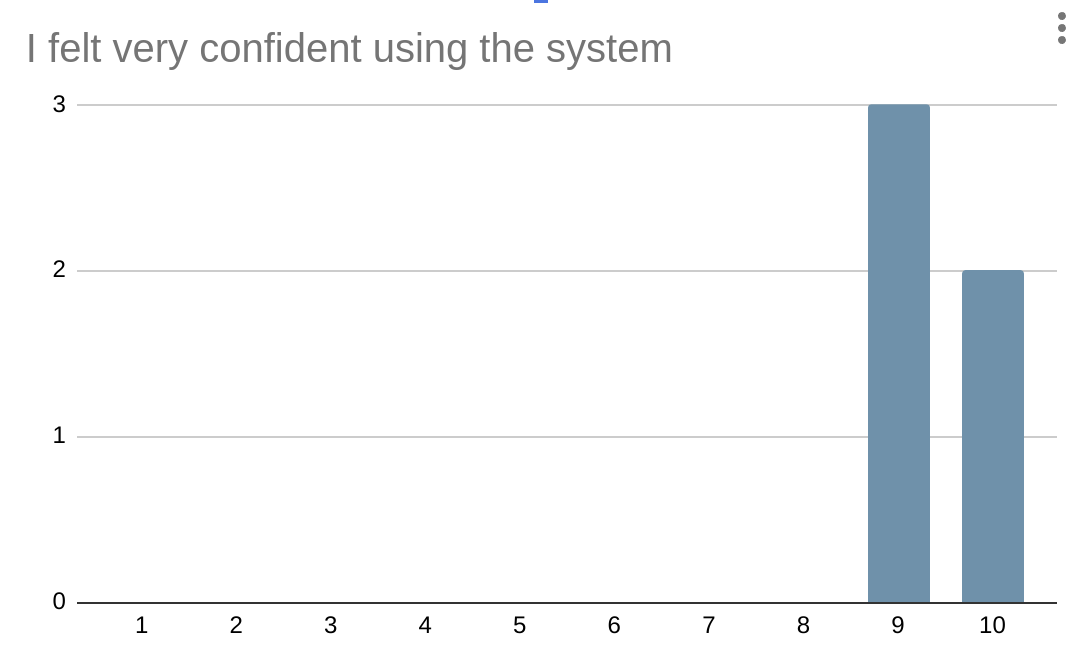
\includegraphics[width=0.8\linewidth]{media/graph_1.png}\\
  \label{image:image-1}
\end{center}

\begin{center}
  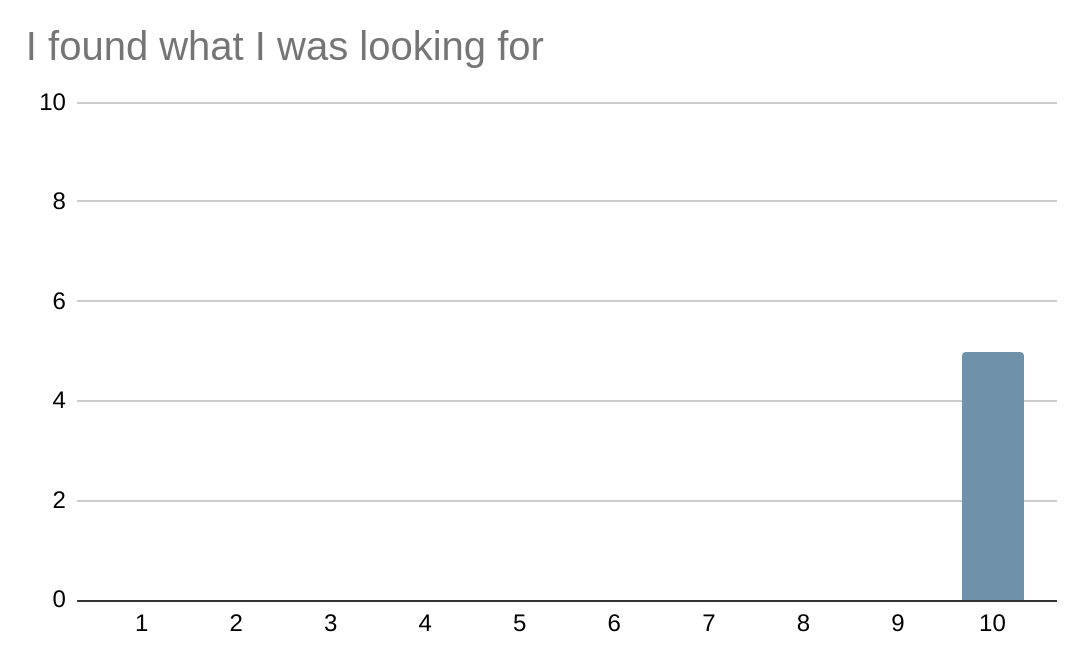
\includegraphics[width=0.8\linewidth]{media/graph_2.png}\\
  \label{image:image-1}
\end{center}

\begin{center}
  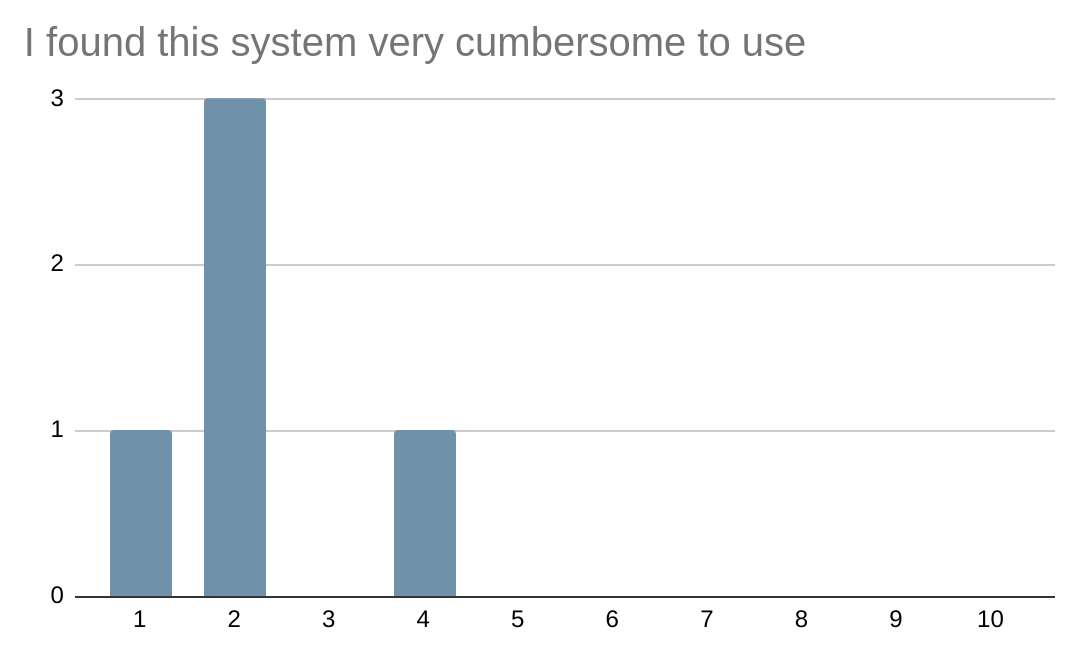
\includegraphics[width=0.8\linewidth]{media/graph_3.png}\\
  \label{image:image-1}
\end{center}

\subsection{Users suggestions}
The comments made by users can be summarised as follows:
\begin{itemize}
    \item the user interface is clean and easy to understand
    \item when the field is not specified the result can be confusing
    \item the results are very tight
    \item the user are in general satisfied with their goal (finding a football team)
\end{itemize}

\section{Figures}
Just put some images of the website
\end{document}
